\subsection{Navarro–Frenk–White profile}

Das Navarro-Frenk-White profil (NFW-profil) ist im grunde genommen eine Funktion
die einem die Warscheinlichkeit das ein Stern an einer bestimmten position ist
liefert.
Die Funktion ist im allgemeinen wie folgt aufgebaut:

\begin{equation}
  \rho = \frac{ 1 }{ \sqrt{ 2 \pi } \cdot \sigma } \cdot
  \exp \left( \frac{ -\phi(r) }{ \sigma^{ 2 } } \right)
\end{equation}

\begin{equation}
  \phi_{NFW}(r) = \frac{ 4\pi \cdot G \cdot f_{0} \cdot R_{s}^3 }{ r } \cdot
  ln{ \left( 1 + \frac{ r }{ R_{s} } \right) }
\end{equation}

Sieht kompliziert aus, ist es aber nicht: Um zu gucken ob ein zufälliger Stern
bei \( x_1 \), \( y_1 \) und \( z_1 \) generiert werden kann wird wie folgt
vorgegangen: Aus den Koordinaten wird der Wert \( r \) mithilfe des Satz des
Phtargoras berechnet, dieser gibt
an wie weit der jeweilige Stern vom Zentrum der Galaxie entfernt ist. Um zu
prüfen ob der Stern generiert wird, wird dieser \( r \)-wert in die Funktion
\( \phi \) eingesetzt. Der entstehende Wert gibt an wie warscheinlich es ist,
das ein Stern in der Entfernung zum Ursprung generiert wird.
\par
Um herrauszufinden ob der Stern generiert wird, wird ein weiterer zufälliger
Wert \( x \) im bereich \( [\phi_{max}; \phi_{min}] \) generiert. Liegt dieser
Wert über dem Wert aus der Funktion \( \phi \) wird kein Stern generiert.
Liegt dieser Stern jedoch unter dem wert aus der \( \phi \) funktion wird
ein Stern an den Koordinaten \( x_1 \), \( y_1 \) und \( z_1 \) generiert.

\subsection{Einasto profile}

\begin{equation}
  \gamma(r) = \frac{ d \ln(\rho(r)) }{ d \ln(\rho) } \propto r^{\alpha}
\end{equation}

\subsection{Blender + Python}

Blender is Awesome, Python is Awesome and together they are
\bold{SUPER AWESOME!!!}

\subsection{Making things faster}

\paragraph{ Kicking out to many Stars, 1 out of 10000 is just to much... }
~\\

\begin{itemize}
  \item Use a custom Density function for each Axis
  \begin{itemize}
    \item \( \phi(r_x)\), \( \phi(r_y) \) and \( \phi(r_z) \)
    \item more controll
  \end{itemize}
\end{itemize}

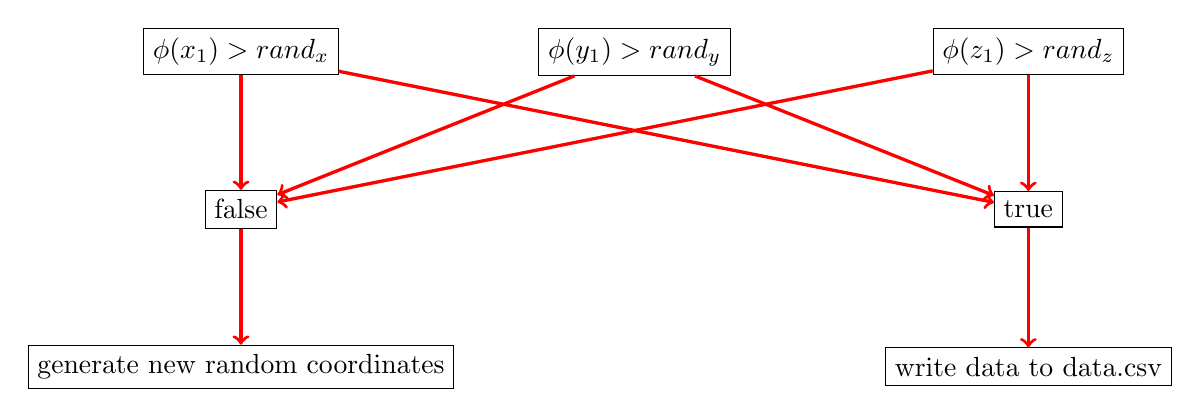
\begin{tikzpicture}
\begin{scope}

    \node[draw] (H) at (0,-2)
        {\( \phi(x_1) > rand_x \)};
    \node[draw] (I) at (5,-2)
        {\( \phi(y_1) > rand_y \)};
    \node[draw] (J) at (10,-2)
        {\( \phi(z_1) > rand_z \)};

    \node[draw] (K) at (10, -4) {true};
    \node[draw] (L) at (0, -4) {false};

    \node[draw] (M) at (10, -6) {write data to data.csv};

    \node[draw] (N) at (0, -6) {generate new random coordinates};

\end{scope}

\begin{scope} [every node/.style={fill=white,circle},
              every edge/.style={draw=red,very thick}]

    \path[->] (H) edge (K);
    \path[->] (I) edge (K);
    \path[->] (J) edge (K);
    \path[->] (H) edge (L);
    \path[->] (I) edge (L);
    \path[->] (J) edge (L);

    \path[->] (K) edge (M);
    \path[->] (L) edge (N);

\end{scope}

\end{tikzpicture}

\subsection{Spiral Galaxies}

The previous Galaxy models where all using a completely spherical model, generating
a spiral galaxy is just not possible using these models.

\subsubsection{N-body problem}

Kurze Beschreibung des N-Körper Problems

\subsubsection{Hilbert Spiral}

Beschreibung der Hilbert Spirale

\subsection{Größeneinheiten}

\begin{equation}
  3.086 \cdot 10^{36} m
\end{equation}
